% !TEX root = ../main.tex
%
\chapter{Appendix A}
\label{sec:appendix}
\nopagebreak
\begin{figure}[ht!]
	\centering
	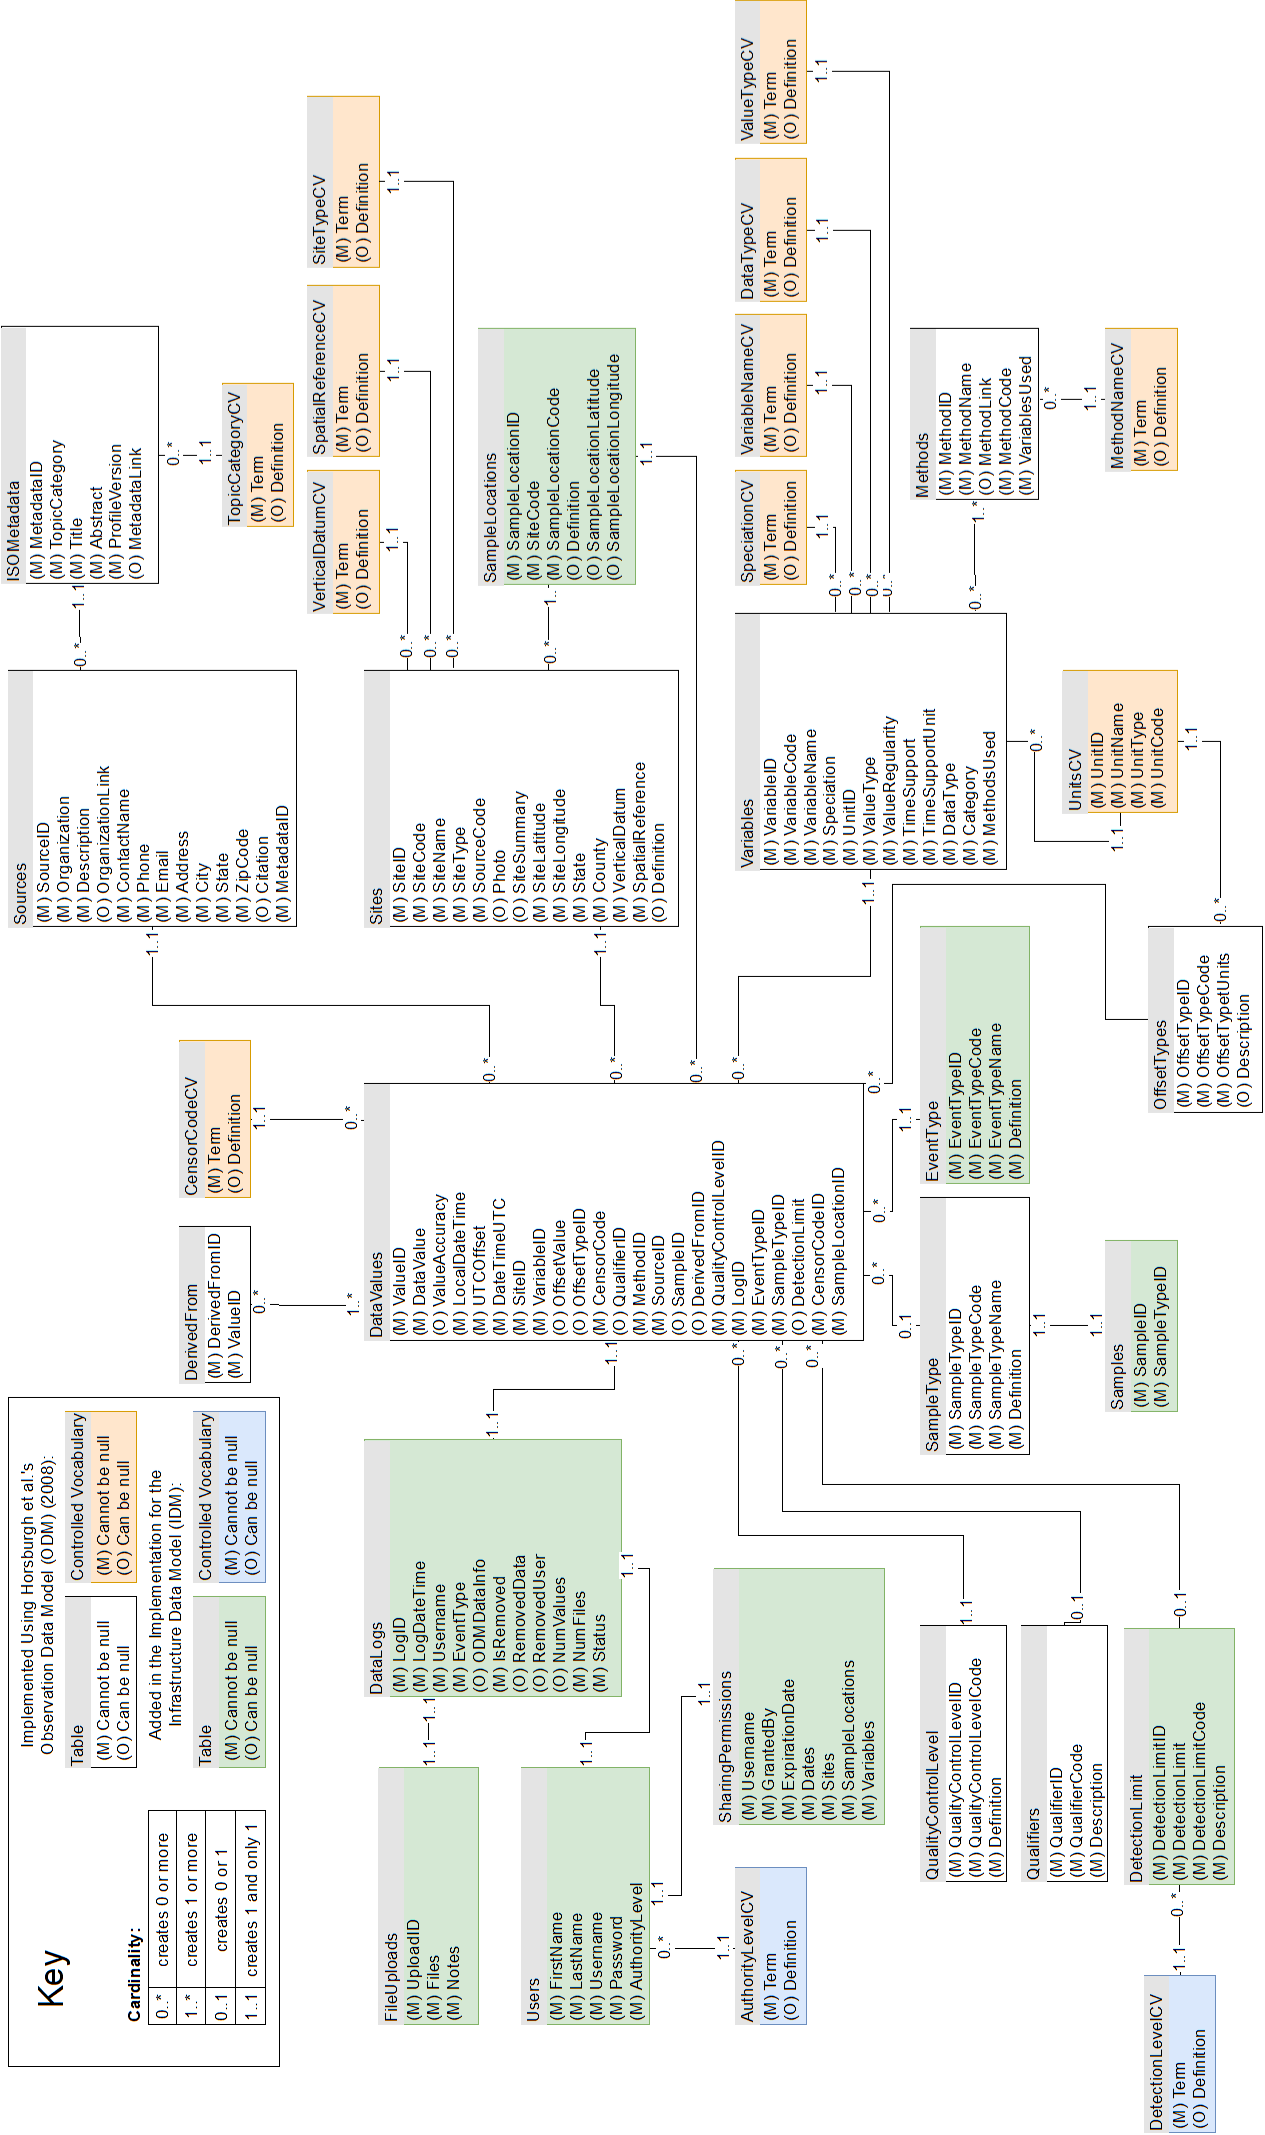
\includegraphics[width=\textwidth, height=0.9\textheight, keepaspectratio]{gfx/chapter-storage/idm_schema_tall.png}
	\caption[SIDM database schema.]{SIDM database schema (Smith et al., submitted).}
\end{figure}


\chapter{Appendix B}

The following R files are also available at \url{www.github.com/andrewkurzweil/MSCE-Thesis/R}.

Data ingest, cleaning, basic event statistics:

%\textit{NOTE: this file is the sole property of the Villanova Center for Resilient Systems and Pennsylvania Department of Transportation as used in monthly reporting. No permissions for outside use are granted and it is provided here for demonstration purposes only.}
\lstinputlisting[lastline = 799]{More-Code/PADOT_DATA_PRE-PROCESSOR_SMP_A.R}
\pagebreak

Ponding recession plots and regression modeling:
\lstinputlisting{../R/04 Recession Modelling.rmd}
\pagebreak

Infiltration timing plots:
\lstinputlisting{../R/05 Recession Timing.rmd}
